\documentclass[aoas,preprint]{imsart}

%% Packages
\RequirePackage{amsthm,amsmath,amsfonts,amssymb}
\RequirePackage[authoryear]{natbib}
\RequirePackage[colorlinks,citecolor=blue,urlcolor=blue]{hyperref}
\RequirePackage{graphicx}

\startlocaldefs
%%%%%%%%%%%%%%%%%%%%%%%%%%%%%%%%%%%%%%%%%%%%%%
%%                                          %%
%% Uncomment next line to change            %%
%% the type of equation numbering           %%
%%                                          %%
%%%%%%%%%%%%%%%%%%%%%%%%%%%%%%%%%%%%%%%%%%%%%%
%\numberwithin{equation}{section}
%%%%%%%%%%%%%%%%%%%%%%%%%%%%%%%%%%%%%%%%%%%%%%
%%                                          %%
%% For Axiom, Claim, Corollary, Hypothezis, %%
%% Lemma, Theorem, Proposition              %%
%% use \theoremstyle{plain}                 %%
%%                                          %%
%%%%%%%%%%%%%%%%%%%%%%%%%%%%%%%%%%%%%%%%%%%%%%
%\theoremstyle{plain}
\newtheorem{axiom}{Axiom}
\newtheorem{claim}[axiom]{Claim}
\newtheorem{theorem}{Theorem}[section]
\newtheorem{lemma}[theorem]{Lemma}
%%%%%%%%%%%%%%%%%%%%%%%%%%%%%%%%%%%%%%%%%%%%%%
%%                                          %%
%% For Assumption, Definition, Example,     %%
%% Notation, Property, Remark, Fact         %%
%% use \theoremstyle{remark}                %%
%%                                          %%
%%%%%%%%%%%%%%%%%%%%%%%%%%%%%%%%%%%%%%%%%%%%%%
\theoremstyle{remark}
\newtheorem{definition}[theorem]{Definition}
\newtheorem*{example}{Example}
\newtheorem*{fact}{Fact}
%%%%%%%%%%%%%%%%%%%%%%%%%%%%%%%%%%%%%%%%%%%%%%
%% Please put your definitions here:        %%
%%%%%%%%%%%%%%%%%%%%%%%%%%%%%%%%%%%%%%%%%%%%%%

\endlocaldefs

\begin{document}

\begin{frontmatter}
\title{A sample article title}
%\title{A sample article title with some additional note\thanksref{t1}}
\runtitle{A sample running head title}
%\thankstext{T1}{A sample additional note to the title.}

\begin{aug}
%%%%%%%%%%%%%%%%%%%%%%%%%%%%%%%%%%%%%%%%%%%%%%
%%Only one address is permitted per author. %%
%%Only division, organization and e-mail is %%
%%included in the address.                  %%
%%Additional information can be included in %%
%%the Acknowledgments section if necessary. %%
%%%%%%%%%%%%%%%%%%%%%%%%%%%%%%%%%%%%%%%%%%%%%%
\author[A]{\fnms{First} \snm{Author}\ead[label=e1]{first@somewhere.com}},
\author[B]{\fnms{Second} \snm{Author}\ead[label=e2,mark]{second@somewhere.com}}
\and
\author[B]{\fnms{Third} \snm{Author}\ead[label=e3,mark]{third@somewhere.com}}
%%%%%%%%%%%%%%%%%%%%%%%%%%%%%%%%%%%%%%%%%%%%%%
%% Addresses                                %%
%%%%%%%%%%%%%%%%%%%%%%%%%%%%%%%%%%%%%%%%%%%%%%
\address[A]{Department,
University or Company Name,
\printead{e1}}

\address[B]{Department,
University or Company Name,
\printead{e2,e3}}
\end{aug}

\begin{abstract}
The abstract should summarize the contents of the paper.
It should be clear, descriptive, self-explanatory and not longer
than 200 words. It should also be suitable for publication in
abstracting services. Formulas should be used as sparingly as
possible within the abstract. The abstract should not make
reference to results, bibliography or formulas in the body
of the paper---it should be self-contained.

This is a sample input file.  Comparing it with the output it
generates can show you how to produce a simple document of
your own.
\end{abstract}

\begin{keyword}
\kwd{First keyword}
\kwd{second keyword}
\end{keyword}

\end{frontmatter}
%%%%%%%%%%%%%%%%%%%%%%%%%%%%%%%%%%%%%%%%%%%%%%
%% Please use \tableofcontents for articles %%
%% with 50 pages and more                   %%
%%%%%%%%%%%%%%%%%%%%%%%%%%%%%%%%%%%%%%%%%%%%%%
%\tableofcontents

\section{Introduction}

This template helps you to create a properly formatted \LaTeXe\ manuscript.
%%%%%%%%%%%%%%%%%%%%%%%%%%%%%%%%%%%%%%%%%%%%%%
%% `\ ' is used here because TeX ignores    %%
%% spaces after text commands.              %%
%%%%%%%%%%%%%%%%%%%%%%%%%%%%%%%%%%%%%%%%%%%%%%
Prepare your paper in the same style as used in this sample .pdf file.
Try to avoid excessive use of italics and bold face.
Please do not use any \LaTeXe\ or \TeX\ commands that affect the layout
or formatting of your document (i.e., commands like \verb|\textheight|,
\verb|\textwidth|, etc.).

\section{Section headings}
Here are some sub-sections:
\subsection{A sub-section}
Regular text.
\subsubsection{A sub-sub-section}
Regular text.

\section{Text}
\subsection{Lists}

The following is an example of an \emph{itemized} list,
two levels deep.
\begin{itemize}
\item
This is the first item of an itemized list.  Each item
in the list is marked with a ``tick.''  The document
style determines what kind of tick mark is used.
\item
This is the second item of the list.  It contains another
list nested inside it.
\begin{itemize}
\item This is the first item of an itemized list that
is nested within the itemized list.
\item This is the second item of the inner list.  \LaTeX\
allows you to nest lists deeper than you really should.
\end{itemize}
This is the rest of the second item of the outer list.
\item
This is the third item of the list.
\end{itemize}

The following is an example of an \emph{enumerated} list of one level.

\begin{longlist}
\item This is the first item of an enumerated list.
\item This is the second item of an enumerated list.
\end{longlist}

The following is an example of an \emph{enumerated} list, two levels deep.
\begin{longlist}
\item[1.]
This is the first item of an enumerated list.  Each item
in the list is marked with a ``tick.''  The document
style determines what kind of tick mark is used.
\item[2.]
This is the second item of the list.  It contains another
list nested inside of it.
\begin{longlist}
\item
This is the first item of an enumerated list that
is nested within.  
\item
This is the second item of the inner list.  \LaTeX\
allows you to nest lists deeper than you really should.
\end{longlist}
This is the rest of the second item of the outer list.
\item[3.]
This is the third item of the list.
\end{longlist}

\subsection{Punctuation}
Dashes come in three sizes: a hyphen, an intra-word dash like ``$U$-statistics'' or ``the time-homogeneous model'';
a medium dash (also called an ``en-dash'') for number ranges or between two equal entities like ``1--2'' or ``Cauchy--Schwarz inequality'';
and a punctuation dash (also called an ``em-dash'') in place of a comma, semicolon,
colon or parentheses---like this.

Generating an ellipsis \ldots\ with the right spacing
around the periods requires a special command.

\subsection{Citation}

Simple author and year cite: \cite{r1}.
Multiple bibliography items cite: \cite{r1,r2}.
Author only cite: \citeauthor{r3}.
Year only cite: \citeyear{r4}.

\section{Fonts}
Please use text fonts in text mode, e.g.:
\begin{itemize}
\item[]\textrm{Roman}
\item[]\textit{Italic}
\item[]\textbf{Bold}
\item[]\textsc{Small Caps}
\item[]\textsf{Sans serif}
\item[]\texttt{Typewriter}
\end{itemize}
Please use mathematical fonts in mathematical mode, e.g.:
\begin{itemize}
\item[] $\mathrm{ABCabc123}$
\item[] $\mathit{ABCabc123}$
\item[] $\mathbf{ABCabc123}$
\item[] $\boldsymbol{ABCabc123\alpha\beta\gamma}$
\item[] $\mathcal{ABC}$
\item[] $\mathbb{ABC}$
\item[] $\mathsf{ABCabc123}$
\item[] $\mathtt{ABCabc123}$
\item[] $\mathfrak{ABCabc123}$
\end{itemize}
Note that \verb|\mathcal, \mathbb| belongs to capital letters-only font typefaces.

\section{Notes}
Footnotes\footnote{This is an example of a footnote.}
pose no problem.\footnote{Note that footnote number is after punctuation.}

\section{Quotations}

Text is displayed by indenting it from the left margin. There are short quotations
\begin{quote}
This is a short quotation.  It consists of a
single paragraph of text.  There is no paragraph
indentation.
\end{quote}
and longer ones.
\begin{quotation}
This is a longer quotation.  It consists of two paragraphs
of text.  The beginning of each paragraph is indicated
by an extra indentation.

This is the second paragraph of the quotation.  It is just
as dull as the first paragraph.
\end{quotation}

\section{Environments}

\subsection{Examples for \emph{\texttt{plain}}-style environments}
\begin{axiom}\label{ax1}
This is the body of Axiom \ref{ax1}.
\end{axiom}

\begin{proof}
This is the body of the proof of the axiom above.
\end{proof}

\begin{claim}\label{cl1}
This is the body of Claim \ref{cl1}. Claim \ref{cl1} is numbered after
Axiom \ref{ax1} because we used \verb|[axiom]| in \verb|\newtheorem|.
\end{claim}

\begin{theorem}\label{th1}
This is the body of Theorem \ref{th1}. Theorem \ref{th1} numbering is
dependent on section because we used \verb|[section]| after \verb|\newtheorem|.
\end{theorem}

\begin{theorem}[Title of the theorem]\label{th2}
This is the body of Theorem \ref{th2}. Theorem \ref{th2} has additional title.
\end{theorem}

\begin{lemma}\label{le1}
This is the body of Lemma \ref{le1}. Lemma \ref{le1} is numbered after
Theorem \ref{th2} because we used \verb|[theorem]| in \verb|\newtheorem|.
\end{lemma}


\begin{proof}[Proof of Lemma \ref{le1}]
This is the body of the proof of Lemma \ref{le1}.
\end{proof}

\subsection{Examples for \emph{\texttt{remark}}-style environments}
\begin{definition}\label{de1}
This is the body of Definition \ref{de1}. Definition \ref{de1} is numbered after
Lemma \ref{le1} because we used \verb|[theorem]| in \verb|\newtheorem|.
\end{definition}

\begin{example}
This is the body of the example. Example is unnumbered because we used \verb|\newtheorem*|
instead of \verb|\newtheorem|.
\end{example}

\begin{fact}
This is the body of the fact. Fact is unnumbered because we used \verb|\newtheorem*|
instead of \verb|\newtheorem|.
\end{fact}

\section{Tables and figures}
Cross-references to labeled tables: As you can see in Table~\ref{sphericcase}
and also in Table~\ref{parset}.

\begin{table*}
\caption{The spherical case ($I_1=0$, $I_2=0$)}
\label{sphericcase}
\begin{tabular}{@{}lrrrrc@{}}
\hline
Equil. \\
points & \multicolumn{1}{c}{$x$}
& \multicolumn{1}{c}{$y$} & \multicolumn{1}{c}{$z$}
& \multicolumn{1}{c}{$C$} & S \\
\hline
$L_1$    & $-$2.485252241 & 0.000000000  & 0.017100631  & 8.230711648  & U \\
$L_2$    & 0.000000000  & 0.000000000  & 3.068883732  & 0.000000000  & S \\
$L_3$    & 0.009869059  & 0.000000000  & 4.756386544  & $-$0.000057922 & U \\
$L_4$    & 0.210589855  & 0.000000000  & $-$0.007021459 & 9.440510897  & U \\
$L_5$    & 0.455926604  & 0.000000000  & $-$0.212446624 & 7.586126667  & U \\
$L_6$    & 0.667031314  & 0.000000000  & 0.529879957  & 3.497660052  & U \\
$L_7$    & 2.164386674  & 0.000000000  & $-$0.169308438 & 6.866562449  & U \\
$L_8$    & 0.560414471  & 0.421735658  & $-$0.093667445 & 9.241525367  & U \\
$L_9$    & 0.560414471  & $-$0.421735658 & $-$0.093667445 & 9.241525367  & U \\
$L_{10}$ & 1.472523232  & 1.393484549  & $-$0.083801333 & 6.733436505  & U \\
$L_{11}$ & 1.472523232  & $-$1.393484549 & $-$0.083801333 & 6.733436505  & U \\
\hline
\end{tabular}
\end{table*}

\begin{table}
\caption{Sample posterior estimates for each model}
\label{parset}
%
\begin{tabular}{@{}lcrcrrr@{}}
\hline
&& & &\multicolumn{3}{c}{Quantile} \\
\cline{5-7}
Model &Parameter &
\multicolumn{1}{c}{Mean} &
Std. dev.&
\multicolumn{1}{c}{2.5\%} &
\multicolumn{1}{c}{50\%}&
\multicolumn{1}{c@{}}{97.5\%} \\
\hline
{Model 0} & $\beta_0$ & $-$12.29 & 2.29 & $-$18.04 & $-$11.99 & $-$8.56 \\
          & $\beta_1$  & 0.10   & 0.07 & $-$0.05  & 0.10   & 0.26  \\
          & $\beta_2$   & 0.01   & 0.09 & $-$0.22  & 0.02   & 0.16  \\[6pt]
{Model 1} & $\beta_0$   & $-$4.58  & 3.04 & $-$11.00 & $-$4.44  & 1.06  \\
          & $\beta_1$   & 0.79   & 0.21 & 0.38   & 0.78   & 1.20  \\
          & $\beta_2$   & $-$0.28  & 0.10 & $-$0.48  & $-$0.28  & $-$0.07 \\[6pt]
{Model 2} & $\beta_0$   & $-$11.85 & 2.24 & $-$17.34 & $-$11.60 & $-$7.85 \\
          & $\beta_1$   & 0.73   & 0.21 & 0.32   & 0.73   & 1.16  \\
          & $\beta_2$   & $-$0.60  & 0.14 & $-$0.88  & $-$0.60  & $-$0.34 \\
          & $\beta_3$   & 0.22   & 0.17 & $-$0.10  & 0.22   & 0.55  \\
\hline
\end{tabular}
%
\end{table}

\begin{figure}
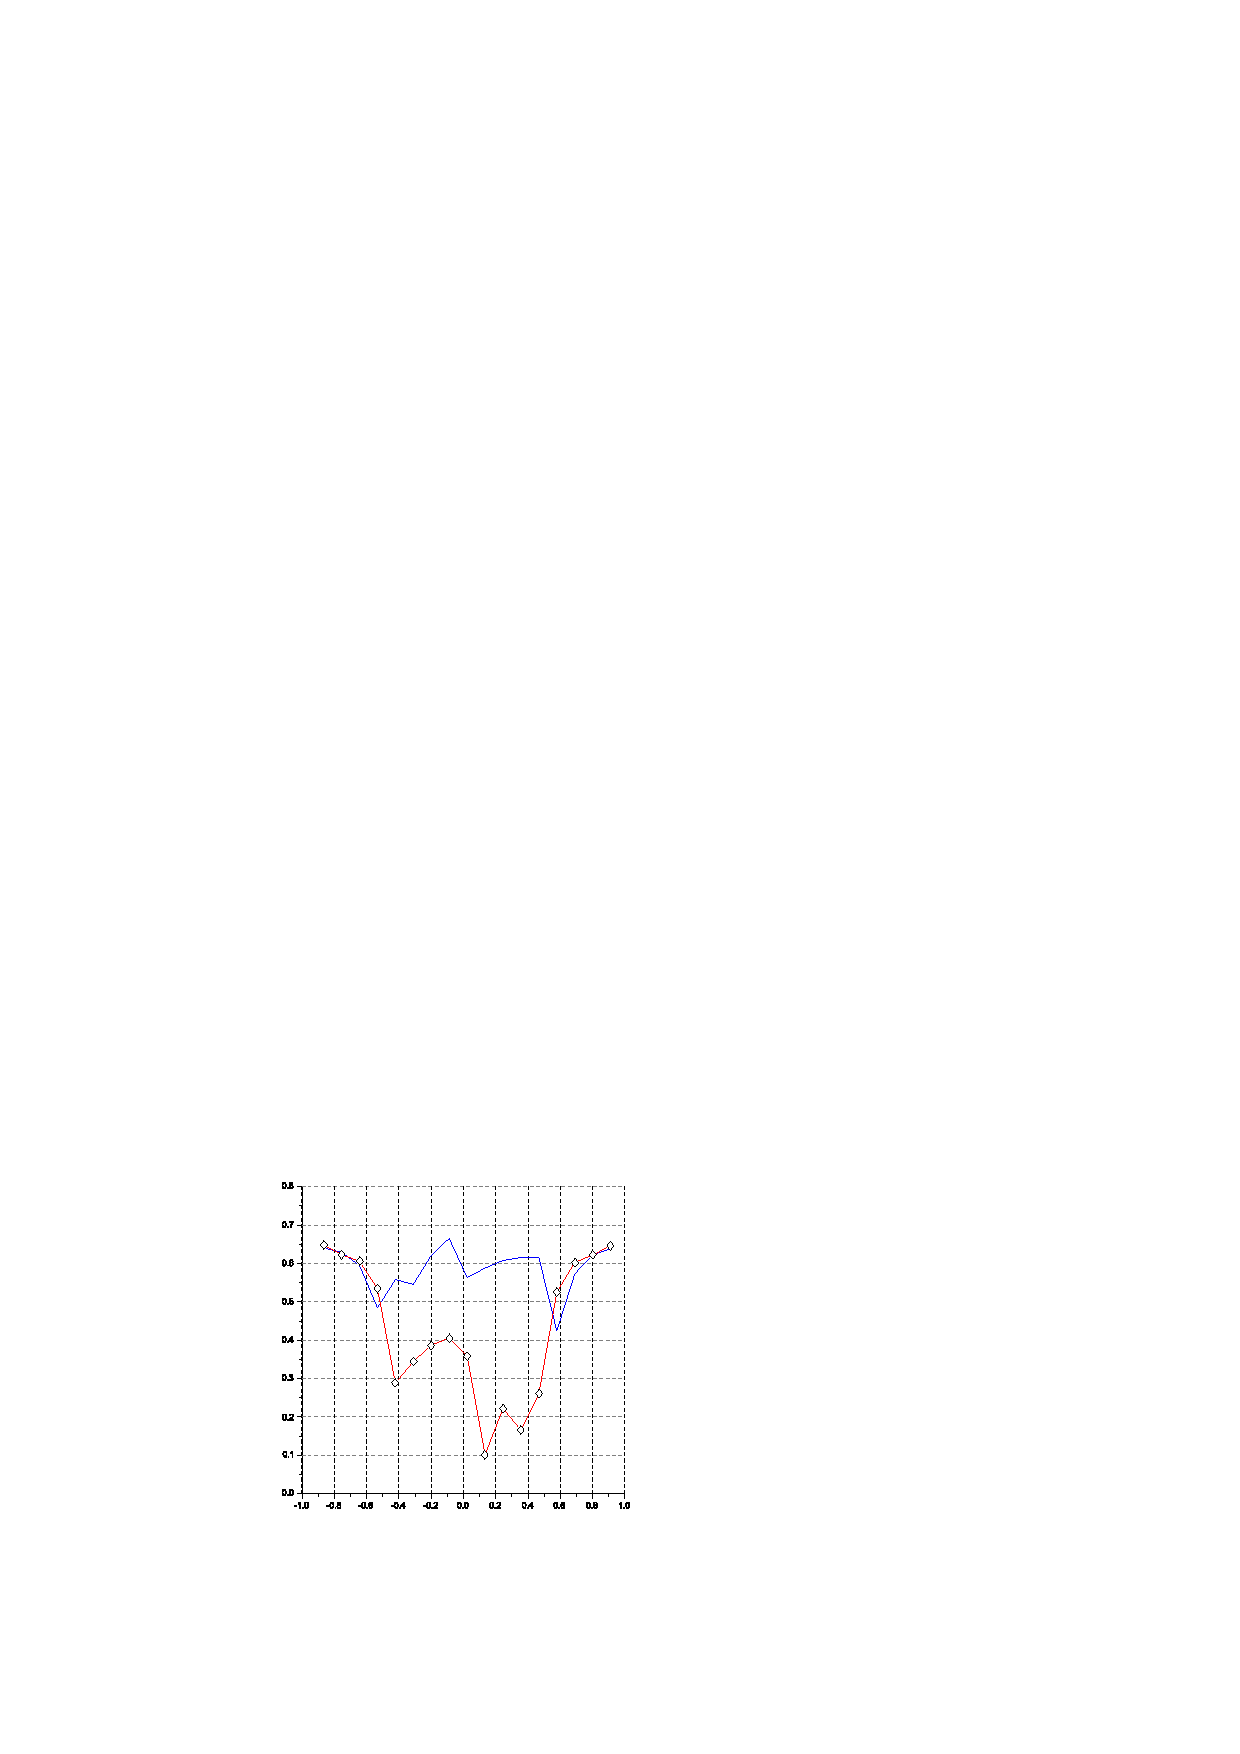
\includegraphics{figure1}
\caption{Pathway of the penicillin G biosynthesis.}
\label{penG}
\end{figure}

Sample of cross-reference to figure.
Figure~\ref{penG} shows that it is not easy to get something on paper.

\section{Equations and the like}

Two equations:
\begin{equation}
    C_{s}  =  K_{M} \frac{\mu/\mu_{x}}{1-\mu/\mu_{x}} \label{ccs}
\end{equation}
and
\begin{equation}
    G = \frac{P_{\mathrm{opt}} - P_{\mathrm{ref}}}{P_{\mathrm{ref}}}  100(\%).
\end{equation}

Equation arrays:
\begin{eqnarray}
  \frac{dS}{dt} & = & - \sigma X + s_{F} F,\\
  \frac{dX}{dt} & = &   \mu    X,\\
  \frac{dP}{dt} & = &   \pi    X - k_{h} P,\\
  \frac{dV}{dt} & = &   F.
\end{eqnarray}
One long equation:
\begin{eqnarray}
 \mu_{\text{normal}} & = & \mu_{x} \frac{C_{s}}{K_{x}C_{x}+C_{s}}  \nonumber\\
                     & = & \mu_{\text{normal}} - Y_{x/s}\bigl(1-H(C_{s})\bigr)(m_{s}+\pi /Y_{p/s})\\
                     & = & \mu_{\text{normal}}/Y_{x/s}+ H(C_{s}) (m_{s}+ \pi /Y_{p/s}).\nonumber
\end{eqnarray}
%%%%%%%%%%%%%%%%%%%%%%%%%%%%%%%%%%%%%%%%%%%%%%
%% Example with single Appendix:            %%
%%%%%%%%%%%%%%%%%%%%%%%%%%%%%%%%%%%%%%%%%%%%%%
\begin{appendix}
\section*{Title}\label{appn} %% if no title is needed, leave empty \section*{}.
Appendices should be provided in \verb|{appendix}| environment,
before Acknowledgements.

If there is only one appendix,
then please refer to it in text as \ldots\ in the \hyperref[appn]{Appendix}.
\end{appendix}
%%%%%%%%%%%%%%%%%%%%%%%%%%%%%%%%%%%%%%%%%%%%%%
%% Example with multiple Appendixes:        %%
%%%%%%%%%%%%%%%%%%%%%%%%%%%%%%%%%%%%%%%%%%%%%%
\begin{appendix}
\section{Title of the first appendix}\label{appA}
If there are more than one appendix, then please refer to it
as \ldots\ in Appendix \ref{appA}, Appendix \ref{appB}, etc.

\section{Title of the second appendix}\label{appB}
\subsection{First subsection of Appendix \protect\ref{appB}}

Use the standard \LaTeX\ commands for headings in \verb|{appendix}|.
Headings and other objects will be numbered automatically.
\begin{equation}
\mathcal{P}=(j_{k,1},j_{k,2},\dots,j_{k,m(k)}). \label{path}
\end{equation}

Sample of cross-reference to the formula (\ref{path}) in Appendix \ref{appB}.
\end{appendix}

%%%%%%%%%%%%%%%%%%%%%%%%%%%%%%%%%%%%%%%%%%%%%%
%% Support information (funding), if any,   %%
%% should be provided in the                %%
%% Acknowledgements section.                %%
%%%%%%%%%%%%%%%%%%%%%%%%%%%%%%%%%%%%%%%%%%%%%%
\section*{Acknowledgements}
The authors would like to thank the anonymous referees, an Associate
Editor and the Editor for their constructive comments that improved the
quality of this paper.

The first author was supported by NSF Grant DMS-??-??????.

The second author was supported in part by NIH Grant ???????????.


%%%%%%%%%%%%%%%%%%%%%%%%%%%%%%%%%%%%%%%%%%%%%%
%% Supplementary Material, if any, should   %%
%% be provided in {supplement} environment  %%
%% with title and short description.        %%
%%%%%%%%%%%%%%%%%%%%%%%%%%%%%%%%%%%%%%%%%%%%%%
\begin{supplement}
\textbf{Title of Supplement A}.
Short description of Supplement A.
\end{supplement}
\begin{supplement}
\textbf{Title of Supplement B}.
Short description of Supplement B.
\end{supplement}

%%%%%%%%%%%%%%%%%%%%%%%%%%%%%%%%%%%%%%%%%%%%%%%%%%%%%%%%%%%%%
%%                  The Bibliography                       %%
%%                                                         %%
%%  imsart-nameyear.bst  will be used to                   %%
%%  create a .BBL file for submission.                     %%
%%                                                         %%
%%  Note that the displayed Bibliography will not          %%
%%  necessarily be rendered by Latex exactly as specified  %%
%%  in the online Instructions for Authors.                %%
%%                                                         %%
%%  MR numbers will be added by VTeX.                      %%
%%                                                         %%
%%  Use \cite{...} to cite references in text.             %%
%%                                                         %%
%%%%%%%%%%%%%%%%%%%%%%%%%%%%%%%%%%%%%%%%%%%%%%%%%%%%%%%%%%%%%

%% if your bibliography is in bibtex format, uncomment commands:
%\bibliographystyle{imsart-nameyear} % Style BST file
%\bibliography{bibliography}       % Bibliography file (usually '*.bib')

%% or include bibliography directly:
\begin{thebibliography}{4}
%%
\bibitem[\protect\citeauthoryear{Billingsley}{1999}]{r1}
\textsc{Billingsley, P.} (1999). \textit{Convergence of
Probability Measures}, 2nd ed.
Wiley, New York.

\bibitem[\protect\citeauthoryear{Bourbaki}{1966}]{r2}
\textsc{Bourbaki, N.}  (1966). \textit{General Topology}  \textbf{1}.
Addison--Wesley, Reading, MA.

\bibitem[\protect\citeauthoryear{Ethier and Kurtz}{1985}]{r3}
\textsc{Ethier, S. N.} and \textsc{Kurtz, T. G.} (1985).
\textit{Markov Processes: Characterization and Convergence}.
Wiley, New York.

\bibitem[\protect\citeauthoryear{Prokhorov}{1956}]{r4}
\textsc{Prokhorov, Yu.} (1956).
Convergence of random processes and limit theorems in probability
theory. \textit{Theory  Probab.  Appl.}
\textbf{1} 157--214.
\end{thebibliography}

\end{document}
